% pagebreak e pentru a termina de desenat toate pozele inainte...
\pagebreak
\section{Interfața de administrare}

	Interfața de administrare nu poate fi accesată dacă nu se cunoaște ori calea, ori dacă nu se navighează din cadrul vizualizării cererii (pentru client, acest pas reprezintă încărcarea pozelor) pe pagina principală.

	Pagina principală a interfeței de administrare se găsește la:

	\begin{verbatim}
	/admin/
	\end{verbatim}

	În momentul în care utilizatorul navighează la \textit{orice} parte a aplicației de administrare și nu este înregistrat, pagina apare ca în figura~\ref{fig:login}.
	\begin{figure}
		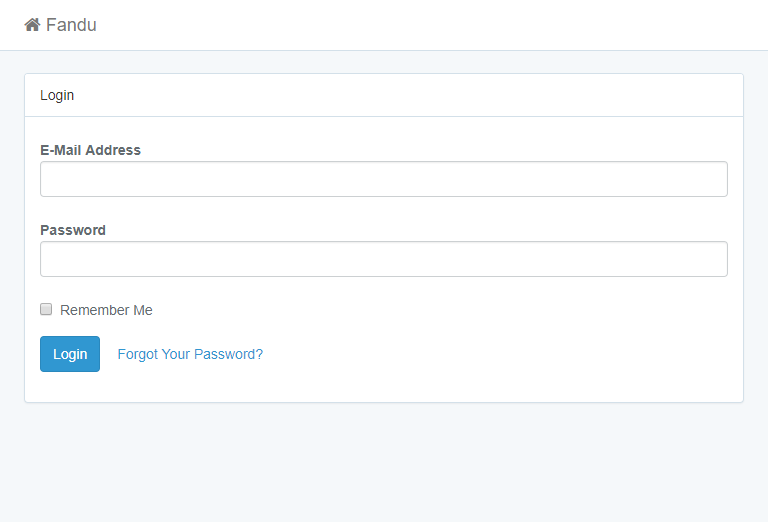
\includegraphics[width=\linewidth]{../imagini/login.png}
		\caption{Pagina de înregistrare pentru interfața de administrare}
		\label{fig:login}
	\end{figure}

	După ce utilizatorul introduce email-ul și parola sa corect în sistem, sistemul va naviga la pagina ce utilizatorul încerca să acceseze.

	Pagina principală a interfeței de administrare arată ca în figura~\ref{fig:home_page}.
	În cazul oricărei probleme, sunt lăsate datele mele de contact pentru a le remedia cât mai rapid.
	De aici, utilizatorul poate introduce rapid un număr de cerere de despăgubire folosind câmpul din bara de navigație.

	În pagina principală, se găsesc două grafice:
	\begin{enumerate}
		\item Primul se referă la cererile de despăgubire noi în această săptămână, raportat la numărul lor pe luna respectivă.
		\item Al doilea se referă la numărul total de decizii terminate, active și refuzate.
	\end{enumerate}

	Numerele folosite în aceste grafice apar atunci când se navighează cu cursorul deasupra lor.

	Bara de navigație conține toate modulele aplicației.

	\begin{figure}
		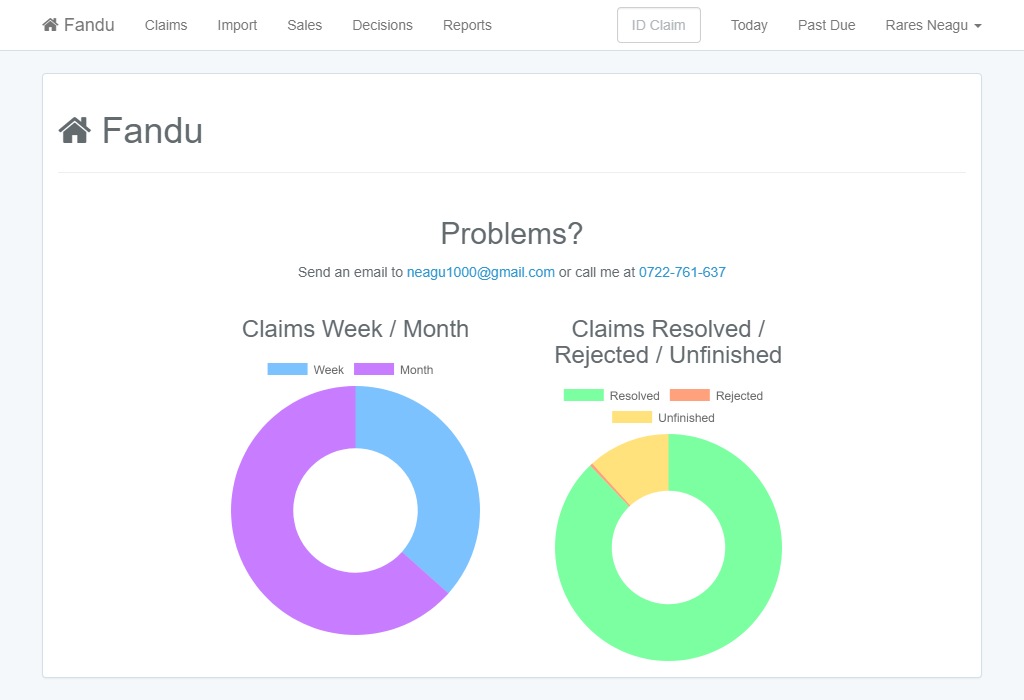
\includegraphics[width=\linewidth]{../imagini/home_page.png}
		\caption{Pagina principală a interfeței de administrare}
		\label{fig:home_page}
	\end{figure}

	\subsection{Claims view}
		\subsubsection{Color code}
		\subsubsection{Search}
			\paragraph{Navbar ID}
		\subsubsection{View claim}
			invoice automatic search
			duplicate imei
			view data
		\subsubsection{Edit Claim}

		\begin{figure}
			\centering
			\subfigure[Fără o decizie - imposibil de modificat] {
				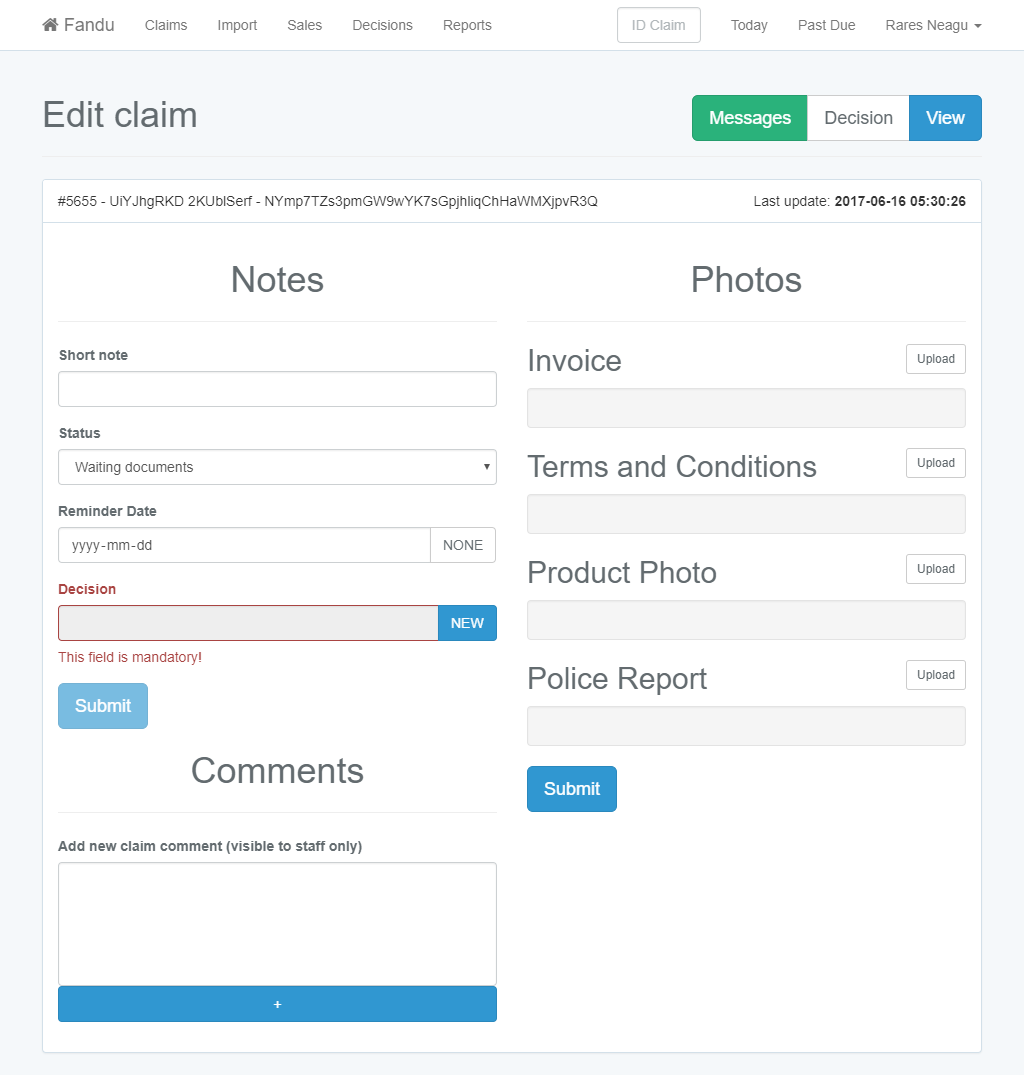
\includegraphics[width=0.4\linewidth]{../imagini/claims_edit.png}
				\label{fig:claims_edit}
			}
			\subfigure[Cu decizie - ușor de modificat] {
				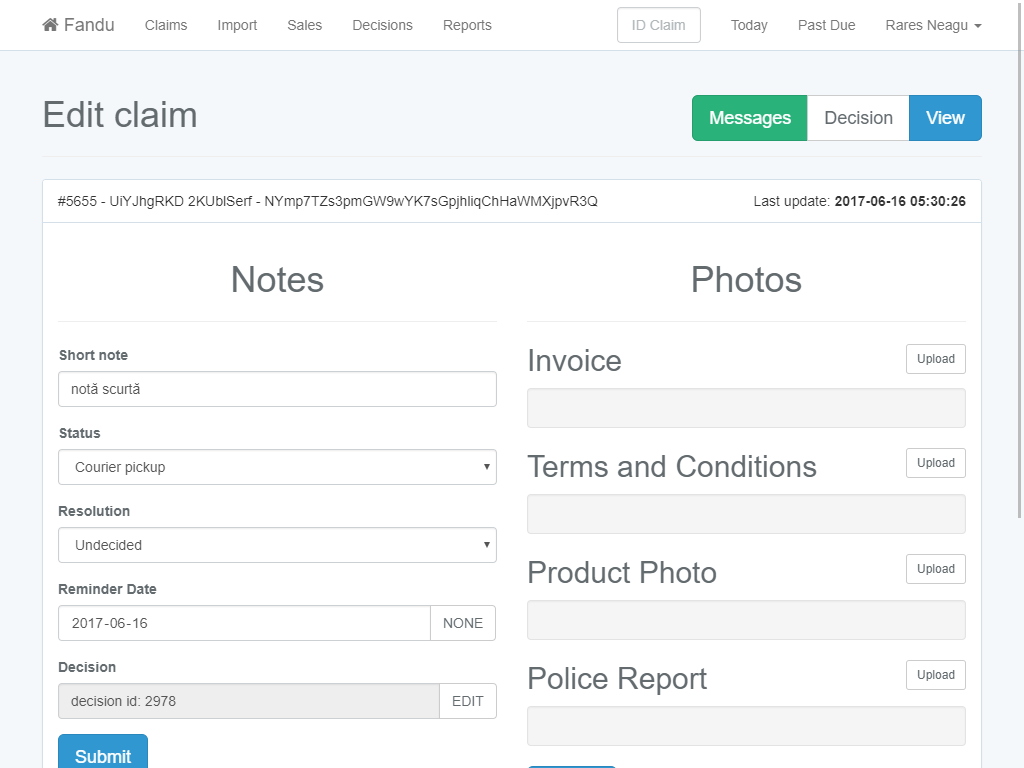
\includegraphics[width=0.4\linewidth]{../imagini/claims_edit_with_decision.png}
				\label{fig:claims_edit_with_decision}
			}
			\caption{Modificarea unei cereri}
		\end{figure}
				short notes
				reminders
				status
				comments
				decisions mandatory - cum / de ce s-a intamplat asta
		\subsubsection{Reminders}
				today
				past due
	\subsection{Import}
		\subsubsection{Weekly Sale import}
			de la altex
		\subsubsection{Custom imports}
			Daily import - format-ul vechi de daily tinut de Ramona pentru fiecare an
			Sales Import - import de date de la "decision" output-ul Fandu (excel stuff) - autocompletare campuri mai mult
			Old - old metadata import from Etonia etc. - ce momentan foloseste doar IMEI
	\subsection{Sales}
		search coloane, access rapid
		buton de remove / remove all logic
		\subsubsection{View}
				poti sa adaugi product
				poti sa stergi product
				poti sa adaugi assurance
				poti sa stergi assurance
	\subsection{Decisions}
		quick search
		detailed search
		de ce poti sa stergi - pentru ca daca nu ai asociat sale-ul corect, poti sa dai undo fara sa sufere nimic baza de date.
		\subsubsection{View}
				claim / messages / add old decision
				edit claim in urma analytics
				campurile explicate
				calculatorul
	\subsection{Reports}
		type of export (deprecated csv / excel)
		date start / end
		progress bar
		metadata when loading - especially yearly reports
		chunking
